% ===================================================================
\section{Population dynamics and chaos (EE03)}
% ===================================================================

\subsection{Why simple models, and what a model is}
Predicting numbers is an old problem (a $\sim$3{,}500-year-old oracle-bone question about locusts; a 1{,}910-year
reconstructed locust index rises and falls irregularly). Nature is complex, so the lecture studies simple models in
order: exponential $\to$ logistic $\to$ cycles and chaos $\to$ ``amelioration'' of chaos. This chapter drops the
structure of EE02 and follows only the total $N$.

\textbf{Rosen's modelling relation.} A natural system $N$ has causal entailment $c$. We \emph{encode} ($\varepsilon$)
part of it into a formal system $F$, \emph{infer} ($i$) consequences by calculation, and \emph{decode} ($\delta$) them
into predictions. The model is good when $\varepsilon\to i\to\delta$ agrees with $c$. When prediction fails, the fault
is in the encoding (a variable was dropped: space, food, age, integer counts) or in the form of the equations, not in
the arithmetic.

\subsection{Exponential growth: the ``first law''}
\[
N_{t+1}=N_t\bigl(1+b-d+i-e\bigr)=\lambda N_t\ \Rightarrow\ N_t=\lambda^tN_0;\qquad
\frac{1}{N}\frac{\dd N}{\dd t}=r\ \Rightarrow\ N=N_0e^{rt};\qquad \lambda=e^{r},\ \ t_d=\frac{\ln 2}{r}.
\]

\begin{keyidea}[: why it is called a law]
It describes a population \emph{in the absence of any external influence}, as Newton's first law describes a body with
no force, and as Hardy--Weinberg describes a gene pool with no evolutionary forces. ``The subject develops by
studying departures from the assumptions.'' The null model is not expected to be true; it is the baseline against
which causes are detected.
\end{keyidea}

Exponential growth has only three behaviours: increase without limit ($r>0$), constancy ($r=0$) or decay to zero
($r<0$). It has \emph{no stable non-zero state}. The doubling time does not depend on $N$. Since real populations
level off, something must make the per-capita rate depend on $N$.

\begin{trap}
$\lambda=e^r$ is exact. What is approximate is $r\approx b-d$ computed from per-step rates: $r=\ln(1+R)\approx R$
only when $R$ is small (June beetle: $R=0.0833$/month gives $r=0.0800$).
\end{trap}

\subsection{Density dependence and the logistic}
Let the realised per-capita rate fall linearly from $r$ at $N=0$ to $0$ at $N=K$: $r'(N)=r(1-N/K)$. Then
\[
\frac{\dd N}{\dd t}=rN\Bigl(1-\frac NK\Bigr),\qquad N(t)=\frac{K}{1+\frac{K-N_0}{N_0}e^{-rt}}.
\]

\begin{center}
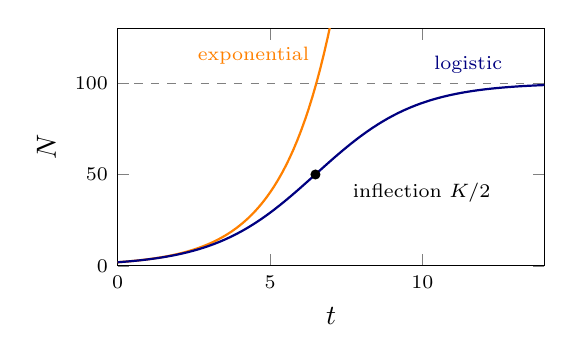
\begin{tikzpicture}
\begin{axis}[width=7cm,height=4.6cm,xlabel={$t$},ylabel={$N$},ymin=0,ymax=130,xmin=0,xmax=14,
  tick label style={font=\scriptsize}]
\addplot[domain=0:7.4,samples=60,thick,orange] {2*exp(0.6*x)};
\addplot[domain=0:14,samples=80,thick,NavyBlue] {100/(1+49*exp(-0.6*x))};
\addplot[dashed,gray] coordinates {(0,100)(14,100)};
\addplot[only marks,mark=*,mark size=1.6pt] coordinates {(6.49,50)};
\node[font=\scriptsize,anchor=west] at (axis cs:7.4,40) {inflection $K/2$};
\node[font=\scriptsize,orange,anchor=east] at (axis cs:6.6,115) {exponential};
\node[font=\scriptsize,NavyBlue] at (axis cs:11.5,110) {logistic};
\end{axis}
\end{tikzpicture}\hspace{4mm}
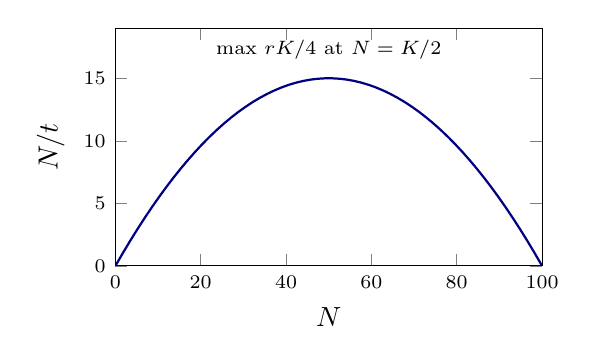
\begin{tikzpicture}
\begin{axis}[width=7cm,height=4.6cm,xlabel={$N$},ylabel={$\dd N/\dd t$},ymin=0,ymax=19,xmin=0,xmax=100,
  tick label style={font=\scriptsize}]
\addplot[domain=0:100,samples=60,thick,NavyBlue] {0.6*x*(1-x/100)};
\node[font=\scriptsize] at (axis cs:50,17.3) {max $rK/4$ at $N=K/2$};
\end{axis}
\end{tikzpicture}
\end{center}

Properties: $N\to K$; the growth rate is a parabola in $N$, largest ($rK/4$) at $N=K/2$, where the curve inflects; fixed
points $0$ (unstable, slope $+r$) and $K$ (stable, slope $-r$); near $K$ deviations decay as $e^{-rt}$, a
\textbf{relaxation time $1/r$}. $K$ is not a number written in the habitat: it is where the realised rate hits zero,
and it moves with food, space or climate.

\textbf{Four ways to write ``rate falls linearly with $N$''} (slide 20), depending on which realised rate is set to
$r(1-N/K)$:
\begin{center}\small
\begin{tabular}{ll}
\toprule
realised rate & model\\\midrule
$\frac1N\frac{\dd N}{\dd t}$ & continuous logistic $\dot N=rN(1-N/K)$\\
$(N_{t+1}-N_t)/N_t$ & discrete logistic $N_{t+1}=N_t[1+r(1-N_t/K)]$\\
$N_{t+1}/N_t$ & ``alternative'' $N_{t+1}=rN_t(1-N_t/K)$ (fixed point $K(1-1/r)$)\\
$\ln(N_{t+1}/N_t)$ & Ricker $N_{t+1}=N_te^{r(1-N_t/K)}$\\\bottomrule
\end{tabular}
\end{center}
Only the continuous one always approaches $K$ smoothly. The data checks (US census, rotifer culture) fit an S-curve
roughly, but slide 23 warns that the realised rate is often \emph{not} linear in $N$: the first few individuals
matter most.

\begin{chain}[: why discrete models can cycle and continuous one-variable models cannot]
A one-variable ODE moves along a line; to oscillate it would have to pass back through a point with the opposite
velocity, which a single-valued $\dot N=f(N)$ forbids. In a discrete map, births come in a pulse once per step, so the
population can \emph{jump over} $K$. A delay acts the same way: in the delayed logistic
$\dot N=rN(t)[1-N(t-\tau)/K]$ the brake responds to an old density, and cycles appear once $r\tau>\pi/2$.
\end{chain}

\subsection{The Ricker model: from stability to chaos}
\[
n_{t+1}=g(n_t)=n_t\exp\!\Bigl[r\Bigl(1-\frac{n_t}{K}\Bigr)\Bigr],\qquad g'(K)=1-r.
\]
$r$ ``determines the qualitative nature of the dynamics''; $K$ is where $n_{t+1}=n_t$ and only rescales ($n=Kx$
removes it).

\begin{chain}[: from the slope at $K$ to the whole route]
\begin{enumerate}
\item For a map, a fixed point is stable iff $|g'(n^*)|<1$: the deviation is multiplied by $g'$ each step.
\item $g'(K)=1-r$. For $0<r<1$ the multiplier is positive: monotone approach. For $1<r<2$ it is negative with
modulus $<1$: the population overshoots each step but by less each time (damped oscillation).
\item At $r=2$ the multiplier passes $-1$: overshoots stop shrinking, and a \textbf{2-cycle} is born.
\item The same thing happens to the 2-cycle (at $r=2.5265$, giving a 4-cycle), then the 4-cycle ($2.6564$, an
8-cycle)\dots: a \textbf{period-doubling cascade} accumulating at $r_\infty\approx2.6924$.
\item Beyond it the dynamics can be \textbf{chaotic}, interspersed with \textbf{periodic windows}.
\end{enumerate}
Biological meaning: \textbf{overcompensation}. At large $r$ a population just below $K$ grows so much it lands
further above $K$ than it was below; each correction is bigger than the error.
\end{chain}

\begin{trap}
Slide 25 labels its $r=2.5$ panel a ``4-point limit cycle''. The Ricker map at $r=2.5$ has period 2 (the 4-cycle lives
in $2.5265<r<2.6564$); a true 4-cycle example is $r=2.6$. If asked, say which value you use.
\end{trap}

\textbf{Bifurcation diagram}: for each $r$, plot the values visited in the long run; the number of points at a given
$r$ is the period. Zooming into it shows smaller copies of the whole (\textbf{fractal}: self-similarity at multiple
scales; slide 26 uses the logistic map's diagram and notes the principle is the same). The ratio of successive gaps
tends to Feigenbaum's constant $4.669$, the same for many one-hump maps (background).

\subsubsection*{Chaos}
\textbf{Deterministic chaos}: bounded, aperiodic behaviour with \textbf{sensitive dependence on initial conditions}.
Nearby starts separate as $\delta_t\approx\delta_0e^{\Lambda t}$ (Lyapunov exponent $\Lambda>0$; Ricker $r=3$:
$\Lambda\approx0.39$). The forecast horizon is $t\approx\ln(\text{range}/\delta_0)/\Lambda$: it grows only
\emph{logarithmically} with measurement precision (a 1000-fold better measurement buys $\ln 1000/0.39\approx18$
generations).

\begin{trap}
Chaos is \emph{not} randomness: no noise enters, and with exact initial values the series is reproducible; what fails
is prediction from imprecise data. Chaos is \emph{not} explosion: the orbit is bounded. And $r>2.69$ does not
guarantee chaos (periodic windows, e.g.\ $r=3.6$). A limit cycle repeats exactly; chaos never repeats.
\end{trap}

\subsection{The real world: Hassell's puzzle and its two resolutions}
\[
N_{t+1}=\lambda N_t(1+aN_t)^{-\beta},\qquad N^*=\frac{\lambda^{1/\beta}-1}{a},\qquad f'(N^*)=1-\beta\bigl(1-\lambda^{-1/\beta}\bigr).
\]
$\beta$ measures how abrupt density dependence is: $\beta\le1$ is \textbf{contest} competition (more parents never mean
fewer offspring; no hump, monotone approach for any $\lambda$); $\beta>1$ is \textbf{scramble} competition (a hump, so
overcompensation is possible). Instability needs both large $\beta$ and large $\lambda$.

Hassell, Lawton and May (1976) fitted $\lambda$ and $\beta$ to 24 insect populations: \textbf{22 of 24 showed monotonic
damping}, so ``natural populations exhibit relatively simple dynamics''. \textbf{The puzzle} (slide 30): simple models
allow chaos at high growth rates, insects have high growth rates, yet except for one or two cases no real population
has been shown to be chaotic, and near-universal simple behaviour ``does not make sense''.

\begin{chain}[: resolution 1, the lattice effect (Henson et al.\ 2001)]
\begin{enumerate}
\item Real organisms come in integers; the models use real numbers.
\item Integer counts with an upper bound give a \emph{finite} set of possible states.
\item A deterministic map on a finite set must eventually revisit a state (pigeonhole), and from then on repeats
exactly. So the integerised model is eventually periodic: \textbf{chaos gives way to limit cycles or extinctions}
(rounding a low point to 0).
\item The number of states grows with $K$, so cycles can be very long (Ricker, $K=10^4$: 82--155 generations). The
lattice effect excludes strict chaos, \textbf{not long-period cycles}, which in finite data look like chaos.
\end{enumerate}
\end{chain}

\begin{chain}[: resolution 2, model complexity (Turchin and Taylor 1992)]
\begin{enumerate}
\item Hassell et al.\ used a model with \textbf{one time lag and a simple functional form}.
\item Real density dependence is often \emph{delayed} (slow food plants, predators building up, cohorts maturing
later), which produces cycles.
\item A one-lag model fitted to such data sees only the average dependence of growth on current density, which slopes
gently down, and reports stability.
\item Fitting many models with more lags and flexible forms found the whole spectrum (damping, oscillatory damping,
limit cycles, chaos). Conclusion: ``use of overly simple models \ldots\ may be \textbf{biased in favour of finding
stability}.''
\end{enumerate}
Slide 35's analogy: a 4-D cube can cast a simple 2-D shadow. Complex high-dimensional objects can have simple
low-dimensional projections, so be careful inferring the object from the shadow.
\end{chain}

\begin{numbers}
Logistic: inflection $K/2$, max rate $rK/4$, relaxation $1/r$. Ricker thresholds: 2 (2-cycle), 2.5265 (4), 2.6564 (8),
2.6924 (chaos). Logistic map: $a=3, 3.449, 3.544,\dots\to3.570$. Hassell: 22/24 monotone. Turchin--Taylor: 14 insect +
22 vertebrate series. Doubling time $\ln 2/r$; human pop.\ doubling in 50\,yr $\Rightarrow r=0.0139$/yr.
\end{numbers}

\begin{statements}
\begin{enumerate}[label=\arabic*.]
\item ``In the Ricker model, raising $K$ can turn a stable population chaotic.''
\F Only $r$ sets the type of dynamics; $K$ rescales.
\item ``The continuous logistic can show damped oscillations if $r$ is large enough.''
\F A one-dimensional ODE cannot oscillate; it approaches $K$ monotonically for any $r>0$. Oscillation needs discrete
steps or delays.
\item ``A population growing logistically adds individuals fastest when it is smallest, because its per-capita rate is highest then.''
\F The per-capita rate is highest at small $N$, but the total rate $rN(1-N/K)$ peaks at $K/2$.
\item ``Chaos and a long limit cycle can both look irregular, but only the cycle repeats exactly.''
\T That is exactly why the lattice effect rules out strict chaos but not long cycles.
\item ``If a chaotic system is deterministic, a better measurement of the initial state will always extend the forecast horizon in proportion.''
\F The horizon grows only with the \emph{logarithm} of precision.
\item ``Hassell et al.'s finding that 22 of 24 populations are monotone shows that chaos is rare in nature.''
\F It shows that a one-lag, simple-form model fitted to the data says so; Turchin and Taylor showed such models are biased toward stability.
\item ``The lattice effect explains why deterministic chaos is not seen, because integer populations with an upper bound have finitely many states.''
\T That is the argument of slide 33 (it says nothing against long cycles).
\item ``The exponential model is useless because no population grows exponentially for long.''
\F It is the null model (``first law''); departures from it are what the subject studies.
\end{enumerate}
\end{statements}

\begin{longans}[: ``Simple models predict chaos at high growth rates, yet chaos is almost never observed. Discuss.'']
(1) Ricker/logistic map: stability for $0<r<2$, period doubling, chaos beyond 2.69; define chaos (deterministic,
bounded, aperiodic, SDIC). (2) Expectation: insects have high $\lambda$, so chaos should be common. (3) Hassell et al.\
1976: 22/24 monotone. (4) Resolution 1, lattice effect: integers + bound $\Rightarrow$ finite states $\Rightarrow$
eventual periodicity or extinction; long cycles still possible. (5) Resolution 2, model complexity: one lag and a
rigid form bias toward stability; Turchin and Taylor's flexible multi-lag fits found the full spectrum including
chaos. (6) Moral: the model is not the world; a low-dimensional projection can hide complex dynamics.
\end{longans}
